\subsubsection{UCS 4 - Modifica dei parametri dell'organizzazione}%kite level

\begin{figure}[h]
	\centering	
	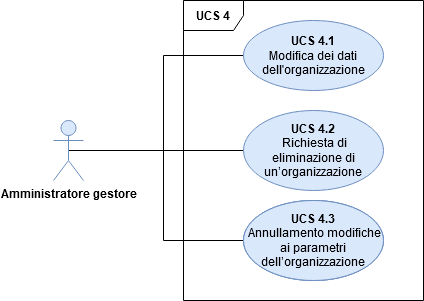
\includegraphics[scale=0.53]{Sezioni/UseCase/Immagini/UCS4.png}
	\caption{UCS 4 - Modifica dei parametri dell'\glo{organizzazione}}
\end{figure}

\begin{itemize}
	\item \textbf{Attori primari:} Amministratore gestore
	\item \textbf{Precondizione:} L'amministratore dispone di almeno un'\glo{organizzazione}.
	\item \textbf{Postcondizione:} L'amministratore ha modificato i parametri desiderati dell'\glo{organizzazione} e le modifiche sono state salvate nel sistema.
	\item \textbf{Scenario principale:} L'amministratore deve scegliere l'\glo{organizzazione} che vuole modificare, selezionare la funzionalità di modifica dell'\glo{organizzazione} e quindi procedere con il cambiamento dei parametri.
	\item \textbf{Scenario alternativo:} L'amministratore non vuole più apportare modifiche all'\glo{organizzazione}, pertanto procederà con l'annullamento dell'apporto di modifiche [UCS 4.3].
	\item \textbf{Flusso di eventi:}
	\begin{enumerate}
		\item L'amministratore seleziona un'\glo{organizzazione} [UCS 3];
		\item L'amministratore seleziona la funzionalità di modifica dell'\glo{organizzazione};
		\item L'amministratore ha la possibilità di modificare i campi delle informazioni dell'\glo{organizzazione} [UCS 4.1];
		\item L'amministratore ha la possibilità di modificare il \glo{perimetro} e i \glo{luoghi} di \glo{tracciamento} dell'\glo{organizzazione} [UCS 5];
		\item L'amministratore seleziona la funzionalità per il salvataggio delle modifiche apportate.
	\end{enumerate}
	\item \textbf{Estensioni:}
	\begin{enumerate}
		\item UCS 4.3 - Annullamento modifiche ai parametri dell'organizzazione.
	\end{enumerate}
\end{itemize}
\newpage
\subsubsection{UCS 4.1 - Modifica dei dati dell'organizzazione}%sea level
\begin{figure}[h]
	\centering
	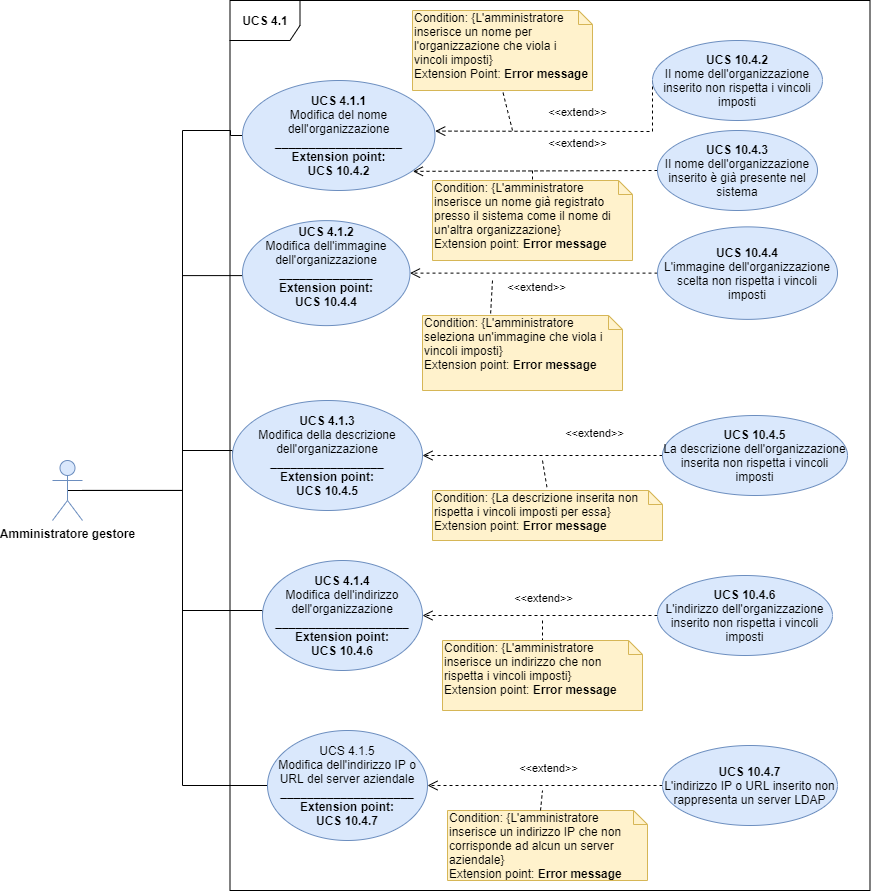
\includegraphics[scale=0.53]{Sezioni/UseCase/Immagini/UCS4.1.png}
	\caption{UCS 4.1 - Modifica dei dati dell'\glo{organizzazione}}
\end{figure}
\begin{itemize}
	\item \textbf{Attori primari:} Amministratore gestore
	\item \textbf{Precondizione:} L'amministratore si trova nella sezione di modifica dei parametri dell'\glo{organizzazione}.
	\item \textbf{Postcondizione:} L'amministratore ha modificato i dati desiderati all'interno dell'\glo{organizzazione}.
	\item \textbf{Scenario principale:} L'amministratore modifica i dati dell'\glo{organizzazione} desiderati, ovvero può:
	\begin{itemize}
		\item modificare il nome dell'\glo{organizzazione} [UCS 4.1.1];
		\item modificare l'immagine dell'\glo{organizzazione} [UCS 4.1.2];
		\item modificare la descrizione dell'\glo{organizzazione} [UCS 4.1.3];
		\item modificare l'indirizzo dell'\glo{organizzazione} [UCS 4.1.4];
		\item modificare l'indirizzo IP o URL del server aziendale [UCS 4.1.5].
	\end{itemize}
\end{itemize}

\subsubsection{UCS 4.1.1 - Modifica del nome dell'organizzazione}%fish level
\begin{itemize}
	\item \textbf{Attori primari:} Amministratore gestore
	\item \textbf{Precondizione:} L'amministratore gestore si trova nella sezione di modifica dei parametri dell'\glo{organizzazione}.
	\item \textbf{Postcondizione:} L'amministratore ha inserito un nome per l'\glo{organizzazione} che rispetti i vincoli imposti e non sia già presente nel sistema.
	\item \textbf{Scenario principale:} L'amministratore modifica il nome dell'\glo{organizzazione}.
	\item \textbf{Scenario alternativo 1:} L'amministratore inserisce un nome per l'\glo{organizzazione} che non rispetta i vincoli imposti. Verrà visualizzato un messaggio d'errore [UCS 10.4.2].
	\item \textbf{Scenario alternativo 2:} L'amministratore inserisce un nome per l'\glo{organizzazione} che è già presente nel sistema. Verrà visualizzato un messaggio d'errore [UCS 10.4.3].
	\item \textbf{Estensioni:}
	\begin{enumerate}
		\item UCS 10.4.2 - Il nome dell'\glo{organizzazione} inserito non rispetta i vincoli;
		\item UCS 10.4.3 - Il nome dell'\glo{organizzazione} inserito è già presente nel sistema.
	\end{enumerate}
\end{itemize}

\subsubsection{UCS 4.1.2 - Modifica dell'immagine dell'organizzazione}%fish level
\begin{itemize}
	\item \textbf{Attori primari:} Amministratore gestore
	\item \textbf{Precondizione:} L'amministratore gestore si trova nella sezione di modifica dei parametri dell'\glo{organizzazione}.
	\item \textbf{Postcondizione:} L'amministratore ha selezionato un'immagine valida per l'\glo{organizzazione}.
	\item \textbf{Scenario principale:} L'amministratore modifica l'immagine dell'\glo{organizzazione}.
	\item \textbf{Scenario alternativo:} L'amministratore seleziona un'immagine per l'\glo{organizzazione} che non rispetta i vincoli imposti. Verrà visualizzato un messaggio d'errore [UCS 10.4.4].
	\item \textbf{Flusso di eventi:}
	\begin{enumerate}
		\item L'amministratore seleziona la funzionalità di scelta dell'immagine;
		\item Seleziona l'immagine da impostare come immagine dell'\glo{organizzazione};
		\item Conferma la scelta.
	\end{enumerate}
	\item \textbf{Estensioni:}
	\begin{enumerate}
		\item UCS 10.4.4 - L'immagine dell'\glo{organizzazione} scelta non rispetta i vincoli imposti.
	\end{enumerate}
\end{itemize}

\subsubsection{UCS 4.1.3 - Modifica della descrizione dell'organizzazione}%fish level
\begin{itemize}
	\item \textbf{Attori primari:} Amministratore gestore
	\item \textbf{Precondizione:} L'amministratore gestore si trova nella sezione di modifica dei parametri dell'\glo{organizzazione}.
	\item \textbf{Postcondizione:} L'amministratore ha inserito una descrizione che rispetti i vincoli imposti.
	\item \textbf{Scenario principale:} L'amministratore modifica la descrizione dell'\glo{organizzazione}.
	\item \textbf{Scenario alternativo:} L'amministratore inserisce una descrizione dell'\glo{organizzazione} che non rispetta i vincoli imposti. Verrà visualizzato un messaggio d'errore [UCS 10.4.5].
	\item \textbf{Estensioni:}
	\begin{enumerate}
		\item UCS 10.4.5 - La descrizione dell'\glo{organizzazione} inserita non rispetta i vincoli.
	\end{enumerate}
\end{itemize}

\subsubsection{UCS 4.1.4 - Modifica dell'indirizzo dell'organizzazione}%fish level

\begin{itemize}
	\item \textbf{Attori primari:} Amministratore gestore
	\item \textbf{Precondizione:} L'amministratore gestore si trova nella sezione di modifica dei parametri dell'\glo{organizzazione}.
	\item \textbf{Postcondizione:} L'amministratore ha inserito un indirizzo valido che rispetti i vincoli imposti.
	\item \textbf{Scenario principale:} L'amministratore modifica l'indirizzo dell'\glo{organizzazione}.
	\item \textbf{Scenario alternativo:} L'amministratore inserisce un indirizzo dell'\glo{organizzazione} che non rispetta i vincoli imposti. Verrà visualizzato un messaggio d'errore [UCS 10.4.6].
	\item \textbf{Flusso di eventi:}
	\begin{enumerate}
		\item L'amministratore inserisce lo stato;
		\item L'amministratore inserisce la città;
		\item L'amministratore inserisce il codice postale;
		\item L'amministratore inserisce una parola tra: via/viale/piazza;
		\item L'amministratore inserisce il nome della via/viale/piazza dell'azienda;
		\item L'amministratore inserisce il numero civico;
		\item Se serve, l'amministratore inserisce la lettera che identifica l'azienda dagli altri edifici che condividono lo stesso numero civico con essa.
	\end{enumerate}
	\item \textbf{Estensioni:}
	\begin{itemize}
		\item UCS 10.4.6 - L'indirizzo inserito non rispetta i vincoli imposti.
	\end{itemize}
\end{itemize}

\subsubsection{UCS 4.1.5 - Modifica dell'indirizzo IP o URL del server aziendale}
\begin{itemize}
	\item \textbf{Attori primari:} Amministratore gestore
	\item \textbf{Precondizione:} L'amministratore gestore si trova nella sezione di modifica dei parametri dell'\glo{organizzazione}.
	\item \textbf{Postcondizione:} L'amministratore ha inserito un \glo{indirizzo IP} o URL valido.
	\item \textbf{Scenario principale:} L'amministratore modifica l'indirizzo del server aziendale.
	\item \textbf{Scenario alternativo:} L'amministratore inserisce un \glo{indirizzo IP} o URL che non rappresenta un server LDAP. Verrà visualizzato un messaggio d'errore [UCS 10.4.7].
	\item \textbf{Flusso di eventi:}
	\begin{enumerate}
		\item L'amministratore inserisce il nuovo \glo{indirizzo IP} o URL.
	\end{enumerate}
	\item \textbf{Estensioni:}
	\begin{itemize}
		\item UCS 10.4.7 - L'indirizzo \glo{IP} o URL inserito non rappresenta un server \glo{LDAP}.
	\end{itemize}
\end{itemize}



\subsubsection{UCS 4.2 - Richiesta di eliminazione di un'organizzazione}%sea level
\begin{itemize}
	\item \textbf{Attori primari:} Amministratore proprietario
	\item \textbf{Precondizione:} L'amministratore si trova nella sezione di modifica dei parametri dell'\glo{organizzazione}.
	\item \textbf{Postcondizione:} L'amministratore ha inviato con successo la richiesta di eliminazione dell'\glo{organizzazione}.
	\item \textbf{Scenario principale:} L'amministratore spiegherà il motivo per cui vuole eliminare l'\glo{organizzazione} e quindi confermerà l'invio della richiesta.
	\item \textbf{Flusso di eventi:}
	\begin{enumerate}
		\item L'amministratore seleziona la funzionalità di richiesta di eliminazione dell'\glo{organizzazione};
		\item L'amministratore inserisce la motivazione che lo ha spinto a richiedere l'eliminazione dell'\glo{organizzazione} [UCS 4.2.1];
		\item L'amministratore seleziona la funzionalità di conferma dell'invio della richiesta di eliminazione dell'\glo{organizzazione}.
	\end{enumerate}
\item \textbf{Inclusione:}
	\begin{itemize}
		\item UCS 4.2.1 - Motivazione della richiesta dell'eliminazione di un'\glo{organizzazione}.
	\end{itemize}
\end{itemize}

\subsubsection{UCS 4.2.1 - Motivazione della richiesta dell'eliminazione di un'organizzazione}%sea level
\begin{itemize}
	\item \textbf{Attori primari:} Amministratore proprietario
	\item \textbf{Precondizione:} L'amministratore si trova nella sezione di modifica dei parametri dell'\glo{organizzazione}.
	\item \textbf{Postcondizione:} L'amministratore ha inserito la motivazione della richiesta di eliminazione dell'\glo{organizzazione}.
	\item \textbf{Scenario principale:} L'amministratore spiegherà il motivo per cui vuole eliminare l'\glo{organizzazione}.
\end{itemize}

\subsubsection{UCS 4.3 - Annullamento modifiche ai parametri dell'organizzazione}%sea level
\begin{itemize}
	\item \textbf{Attori primari:} Amministratore gestore
	\item \textbf{Precondizione:} L'amministratore gestore si trova nella sezione di modifica dei parametri dell'\glo{organizzazione}.
	\item \textbf{Postcondizione:} L'amministratore ha annullato le modifiche ai parametri dell'\glo{organizzazione}.
	\item \textbf{Scenario principale:} L'amministratore procederà ad annullare le modifiche ai parametri dell'\glo{organizzazione} che sta apportando.
	\item \textbf{Flusso di eventi:}
	\begin{enumerate}
		\item L'amministratore seleziona la funzionalità per annullare le modifiche e tornare alla sezione di gestione dell'\glo{organizzazione}.
	\end{enumerate}
	\item \textbf{Inclusioni:}
	\begin{enumerate}
		\item UCS 10.4.1 - Visualizzazione del messaggio di conferma di annullamento modifiche.
	\end{enumerate}
\end{itemize}